\chapter{Simple Pendulum}

\section{Aim}
To investigate the relationship between the length of a simple pendulum and the period of its oscillations

\section{Background Information}
A simple pendulum is a weight suspended from a point by a light non stretchable string so that the weight can swing freely. A simple pendulum is very useful for clocks, the calculation of the acceleration due to gravity, and other scientific instruments. This is because the time it takes for a pendulum to swing back and forth is relatively constant. In order to design a pendulum to give the desired time of oscillation we must learn which variables effect this periodic time. It is possible the length of the pendulum affects the period of oscillation so we should investigate this relationship. 

\section{Materials}
Retort stand, meter rule, stop watch, string about 150 cm long, 2 wood pads and a pendulum bob

\section{Procedure}
\begin{enumerate}
\item Tie a pendulum bob to one end of a string.
\item Clamp the other end of the string firmly between the two wooden pads on the retort stand so that the length $L$ of the string is 100 cm.
\item Displace the pendulum bob by a small angle and release it. Record the time, $t$, in seconds for twenty (20) oscillations.  
\item Repeat procedure (3) for the values of $L$ of 80 cm, 60 cm, 40 cm and 20 cm.
\end{enumerate}


\begin{figure}[h!]
\centering
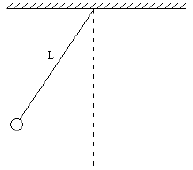
\includegraphics[width=6cm]{./img/pendulum-1.png}
\caption{Simple Pendulum practical setup}
\label{fig:pendulum-1}
\end{figure}

\section{Analysis and Interpretation}
\begin{enumerate}
\item Tabulate your results as $L$, $t$, period $T$ and $T^2$, whereby the period is the total time divided by the total number of oscillations to give the time per oscillation.
\item Plot the graph of $L$ against $T^2$. 
\item Draw a best-fit line and determine its slope.
\end{enumerate}

\section{Conclusion}
What is the relationship between the length of a pendulum and its period of oscillation?

\section{Questions for Discussion}
\begin{enumerate}
\item Given that $T=2\pi(^L/_g)^{^1/_2}$  find the value of $g$ from your experiment.
\item What would be the relationship between $L$ and $T^2$ if the graph of $T^2$ is plotted against $L$?
\item Do you think the mass and the shape of the pendulum bob affects the period of oscillation? 
\item Will two pendulums of the same length have the same period if they are at two different altitudes? Explain.
\end{enumerate}

\section{Reflection and Self Assessment}
\begin{enumerate}
\item What did you find most and least interesting about this experiment? Explain.
\item What is the significance of ‘$g$’ in our daily life?
\item Is there anything you do not understand about this experiment? If so, what is it and in what ways can you improve your understanding?
\end{enumerate}